\capitulo{3}{Conceptos teóricos}

\section{Minería de datos}

La minería de datos consiste en la aplicación de técnicas de la inteligencia artificial sobre grandes volúmenes de datos, teniendo como objetivo el extraer tendencias o patrones interesantes de dicho conjunto de datos y convertirlos en un formato comprensible.

Todos los días se crea una gran cantidad de bytes de datos, pero para extraer información singular de esos datos es necesario aplicar distintos métodos o técnicas tales como el aprendizaje automático. Para ello se llevan a cabo distintas etapas \cite{MD:tecnicasyherramientas}:

\begin{itemize}
    \item \textbf{Selección:} Recopilar e integrar los volúmenes de datos existentes. Identificar las variables más importantes. Aplicar técnicas de muestreo.
    \item \textbf{Exploración:} Utilizar las técnicas de análisis de exploratorio de datos. Obtener la distribución de los datos. Analizar la conexión que existe dentro de esta información.
    \item \textbf{Limpieza:} Detección de valores atípicos. Eliminar datos erróneos e irrelevantes.
    \item \textbf{Transformación:} Modificar la dimensión (aumentar, disminuir). Utilizar técnicas de discretización y numeración. Creación del escalado simple y multidimensional.
    \item \textbf{Minería de datos:} Utilizar técnicas predictivas: análisis discriminante, redes neuronales, árboles de decisión, regresión y series temporales, algoritmos genéticos y métodos bayesianos. Utilizar técnicas descriptivas: Reglas de asociación y dependencia, \textit{Clustering} y segmentación, reducción de la dimensión, escalamiento y análisis explorativo.
    \item \textbf{Evaluación e interpretación de resultados:} Intervalos de confianza, \textit{bootstrap}, análisis ROC\footnote{ Representación de la razón o ratio de verdaderos positivos (VPR) frente a la razón o ratio de falsos positivos (FPR) según se varía el umbral de discriminación.} (\textit{Receiver Operating Characteristic}), evaluación de modelos.
    \item \textbf{Difusión y uso de modelos:} Su visualización y su simulación.
\end{itemize}

Esto tiene relación con este proyecto porque disponemos de unas imágenes de las que queremos obtener una información en concreto. Por lo tanto, en nuestro caso como ya disponemos de las imágenes solo aplicaremos las tres últimas etapas.

Ahora definiremos algunos conceptos importantes para entender mejor todo esto.

\subsection{Inteligencia Artificial}

La inteligencia artificial o IA es la simulación de tareas intelectuales realizadas por humanos por parte de las máquinas, es decir, es una disciplina que es capaz de crear sistemas con capacidad de aprender según su experiencia como una persona real, siendo también capaces de resolver problemas o llevar a cabo tareas lógicas.

La inteligencia artificial contiene el aprendizaje automático (\textit{Machine Learning}) y el aprendizaje profundo (\textit{Deep Learning}) aunque también es parte de campos que no llevan a cabo un aprendizaje como tal.

Durante los años 80 se pensaba que se podía alcanzar al nivel de inteligencia humana haciendo que los programadores crearan un gran conjunto de reglas suficiente para controlar el conocimiento y construir máquinas intelectuales. Esta idea es conocida como \textit{IA simbólica}.

Se comprobó que este enfoque era capaz de resolver problemas que estaban bien definidos y eran lógicos, como jugar al ajedrez, pero no era funcional con problemas más complejos que necesitaban reglas explícitas para su resolución, como el reconocimiento de voz, la clasificación de imágenes, etc. Para estos problemas se trató con un nuevo enfoque, el aprendizaje automático o \textit{machine learning}.

\begin{figure}[htb]
	\centering
	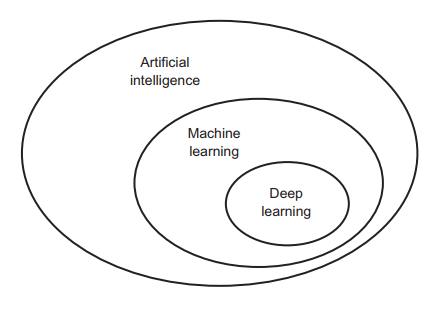
\includegraphics[width=0.7\textwidth]{IA_AA_AP}
	\caption[Inteligencia Artificial y subcampos]{Inteligencia Artificial y subcampos \cite{MD:aprendizajeautomatico}}
\end{figure}


Sobre la selección de las imágenes en este proyecto no hay una selección en sí de imágenes para el entrenamiento y el testeo, sino que hay un archivo tipo .txt que contiene la dirección de las imágenes que se van a entrenar y otro con las que se van a testear.

\subsection{Aprendizaje Automático o \textit{Machine Learning}}

A la mayoría de los programas se les introducen unas reglas y unos datos para que sean procesados siguiendo estrictamente estas reglas y de este modo se obtiene una o varias respuestas al final del programa, pero con el aprendizaje automático son los datos y sus respuestas esperadas, en el caso del aprendizaje supervisado, lo que se introduce como entrada con el fin de obtener las reglas que permitan hacer un mapeo efectivo. Estas reglas son las que a continuación van a ser utilizas con un nuevo conjunto de datos para generar sus respuestas, es decir, el sistema ``ha aprendido'' a generar estas respuestas.

Por lo tanto, para la poder realizar un aprendizaje automático necesitamos tres componentes indispensables:

\begin{itemize}
    \item \textbf{Datos de entrada:} En nuestro caso imágenes de rayos-X de piezas metálicas con o sin defectos.
    \item \textbf{Datos salida esperados:} La localización de los defectos de cada imagen. En nuestro proyecto tenemos las máscaras de las imágenes y los \textit{bounding box} (cuadro delimitador) donde se encuentran los errores.
    
    Las máscaras son imágenes de ceros y unos, los unos representan el pixel donde se encuentra un defecto y los ceros el resto de la imagen.
    
    \imagen{imagen_prueba}{Imagen de prueba\label{imagen_prueba}}
    
    \imagen{mascara_prueba}{Máscara de una imagen de prueba\label{mascara_prueba}}
    
    En la figura \ref{imagen_prueba} tenemos una imagen con los defectos superpuestos y en la figura \ref{mascara_prueba} se ve la máscara de uno de los defectos de la imagen, los pixeles blancos representan un defecto.
    
    El \textit{bounding box} de esta imagen es: [(472, 171, 493, 199)]. Estos valores representan las \textit{x} y las \textit{y} de donde se encuentra el defecto ([(xmin, ymin, xmax, ymax)]).
    \item \textbf{Un método de comprobación de la salida generada:} Imprescindibles para determinar la diferencia entre la salida generada y la salida esperada. Esto se utiliza como señal realimentación para que el algoritmo se actualice o aprenda.
\end{itemize}

Estos componentes también son los imprescindibles en el aprendizaje profundo. Los tipos de implementación son \cite{MD:machinelearning}:

\begin{itemize}
	\item \textbf{Aprendizaje supervisado:} Los algoritmos disponen de datos ``etiquetados'' (\textit{labelled data}) e intentan crear una función que, dados los datos de entrada, asigne una etiqueta adecuada a los datos de salida. El algoritmo va a aprender a asignar las etiquetas gracias a un conjunto de datos pre-existente con el que se entrena.
	\item \textbf{Aprendizaje no supervisado:} Los algoritmos no disponen de datos ``etiquetados'', solo se conoce los datos entrada, no existen las etiquetas asociadas que permiten establecer la clase a la que pertenecen. Es decir, intentan descubrir la estructura de los datos para encontrar alguna forma de organización o patrón.
	\item \textbf{Aprendizaje de refuerzo:} La base de este tipo de aprendizaje es mejorar la respuesta del modelo. Para ello lleva a cabo un proceso de retroalimentación, es decir, aprende del medio externo, del entorno que le rodea. Los datos de entrada son los \textit{feedback} que obtiene como respuesta a sus acciones. El sistema aprende a base de ensayo-error.
\end{itemize}

\subsection{Aprendizaje Profundo o \textit{Deep Learning}}

Este tipo de aprendizaje se basa en la creación de modelos computacionales compuestos por varias capas, es decir, el término ``profundo'' hace referencia a la idea de la representación continua de los datos por medio de dichas capas. La profundidad del modelo es la cantidad de capas que tenga.

Los modelos de estas capas son denominados \textbf{Redes Neuronales}, las capas están apiladas una detrás de la otra. Este término viene de la neurobiología, y aunque muchos de los conceptos del aprendizaje profundo tuvieron como inspiración el funcionamiento del cerebro humano, la verdad es que aún no hay evidencias de que el cerebro esté estructurado de esta forma ni de que aprenda usando estos modelos de aprendizaje profundo.

\subsubsection{Redes Neuronales}

Como ya hemos dicho este algoritmo está basado en el funcionamiento del cerebro humano, es decir, que entre las capas o nodos denominados neuronas artificiales se transmiten señales entre sí desde la capa de entrada (\textit{input}) hasta la de salida (\textit{output}). Dentro de cada neurona hay a su vez capas que poseen un peso, un valor numérico con el que modifica su entrada. La capa pasa al siguiente la salida que ha obtenido y así hasta el final.

\imagen{EsquemaRedNeuronal}{Funcionamiento esquematizado de las Redes Neuronales}

\section{Nondestructive testing (NDT)}

El \textit{Nondestructive testing} (NDT) \cite{NDT} es un procedimiento que se usa para inspeccionar, probar o evaluar los materiales o componentes para detectar defectos en las características de tal manera que la estructura o diseño original de estos materiales al ser inspeccionados no sean modificados o destruidos. Al final de la inspección, la pieza no debe haber sido modificada, debe poder usarse.

Este tipo de pruebas se hacen para asegurar que la calidad de los productos alcance un cierto ``estándar''.

Para las pruebas destructivas debe haber un número limitado de componentes de muestra en vez de los componentes que realmente van a salir al mercado. Estas pruebas se suelen utilizar en la fabricación para garantizar la fiabilidad del producto, reducir costes de producción y mantener un alto nivel de calidad.

Hay tres tipos de métodos de pruebas:
\begin{itemize}
    \item \textbf{Superficiales:} Dan información sobre el estado superficial de los materiales inspeccionados. Los métodos son: Inspección Visual (VT), Líquidos Penetrantes (PT), Partículas Magnéticas (MT) y Electromagnetismo (ET).
    \item \textbf{Volumétricas:} Dan información sobre el estado interno de los materiales inspeccionados. Los métodos son: Radiografía Industrial (RT), Ultrasonido Industrial (UT) y Emisión Acústica (AE).
    \item \textbf{De hermeticidad:} Dan información del grado en que pueden ser contenidos los fluidos en recipientes, los métodos son: Pruebas de Fuga, Pruebas por Cambio de Presión (neumática o hidrostática), Pruebas de Burbuja, Pruebas por Espectrómetro de Masas y Pruebas de Fuga con Rastreadores de Halógeno.
\end{itemize}

Para este proyecto trabajaremos con radiografías industriales (\textit{Radiographic Testing} o RT) que utilizan rayos-X o rayos-gamma. Las aleaciones de aluminio son ligeras y poco densas por lo que es mejor utilizar rayos-X, los rayos-gamma se suelen utilizar para metales más gruesos o densos como el plomo o el hormigón.

\subsection{Radiografías Industriales (RT)}

Este método de pruebas implica que un objeto de prueba va a ser expuesto a una gran radiación que pasará a través de él y genera una imagen en una placa especial.

Las placas que se suelen utilizar se llaman películas de rayos-X industriales, también se pueden utilizar algunos tipos de detectores de radiación digital. El efecto final de tener áreas más claras, donde la radiación ha penetrado menos, y áreas más oscuras, donde la radiación ha pasado más fácilmente. Si hay un defecto o vacío en una parte donde pasa más radiación se queda plasmado en la película como una mancha oscura.

\begin{figure}[htb]
	\centering
	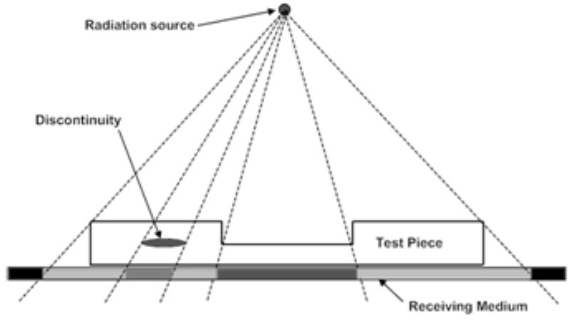
\includegraphics[width=0.9\textwidth]{NDT_RT}
	\caption[Ejemplo de radiografías industriales]{Ejemplo de radiografías industriales \cite{NDT}}
\end{figure}

\section{Segmentación de imágenes}

Consiste en dividir la imagen en sus partes componentes hasta llegar a un punto de subdivisión en el que se recogen las regiones u objetos de interés. La base de estos algoritmos es o la similitud o la discontinuidad entre los niveles de gris (en las imágenes que sean en escala de grises) o entre valores RGB (en las imágenes a color) de píxeles vecinos.

Este proyecto ha utilizado el modelo de \textit{deep learning} \textbf{Mask R-CNN} \cite{segmentacionimagenes:MaskR-CNN} para la detección de defectos en piezas metálicas. Esta implementación parte del \textit{framework} realizado por Matterport Inc. \cite{segmentacionimagenes:MaskR-CNN2}, el cual se proporciona en código abierto.

\subsection{Mask R-CNN}

Las redes neuronales convolucionales son  un tipo de redes neuronales artificiales  donde las “neuronas”  corresponden a campos receptivos de una manera muy similar a las neuronas en la corteza visual primaria de un cerebro biológico.

Mask R-CNN es una red neuronal convolucional regional que se compone de un marco de dos etapas: la primera escanea la imagen y genera propuestas (áreas que probablemente contengan un objeto). La segunda clasifica las propuestas y genera cuadros delimitadores y máscaras.

\begin{figure}[htb]
	\centering
	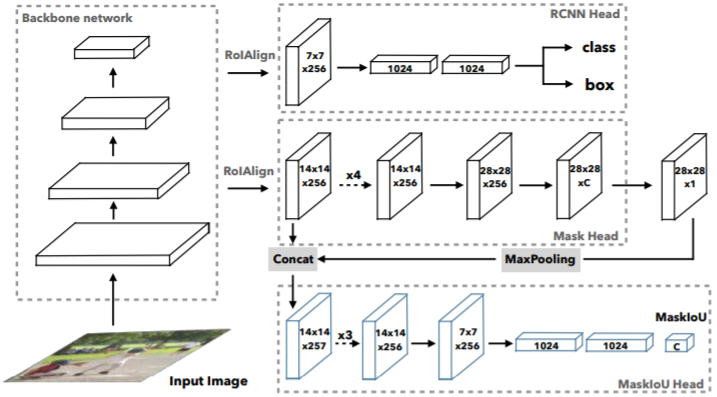
\includegraphics[width=0.9\textwidth]{mascara_layers}
	\caption[Arquitectura de red de la máscara R-CNN]{Arquitectura de red de la máscara R-CNN \cite{segmentacionimagenes:mascara_layers}}
\end{figure}

La primera etapa de esta arquitectura contiene tres sub-bloques:

\begin{itemize}
    \item \textbf{\textit{Backbone}:} Se encarga de extraer mapas de características de las imágenes con capas convolucionales (normalmente ResNet50 o ResNet101 \ref{resnetLabel}).
    \item \textbf{\textit{Feature Pyramid Network} (FPN) \cite{segmentacionimagenes:FPN}:} Permite que las características de alto nivel se encuentren a diferentes escalas y con información de diferentes niveles.
    \item \textbf{\textit{Region Proposal Network} (RPN) \cite{segmentacionimagenes:RPN}:} Propone regiones que tienen una alta probabilidad de contener un objeto de una de las clases entrenadas.
\end{itemize}

ResNet\label{resnetLabel} (\textit{Residual neural network}) \cite{ResNet} es un tipo de red neuronal convolucional, que se utiliza frecuentemente para clasificar imágenes, también es capaz de extraer características de dichas imágenes. Los detalles del modelo ResNet son:

\begin{itemize}
    \item \textbf{Etapa 1:} La convolución 2D tiene 64 filtros de forma\footnote{\textit{Kernel size} o tamaño del grano de la imagen.} (7,7) y utiliza una zancada\footnote{\textit{Strides} o saltos, se utilizan para reducir la carga de anclajes. Si generamos anclajes para cada otra celda en el mapa de características y tenemos una zancada de 2 el número de anclas se reducirá en 4.} de (2,2). Su nombre es ``conv1''. \textit{BatchNorm}\footnote{Es una técnica para mejorar la velocidad, el rendimiento y la estabilidad de las redes neuronales artificiales.} se aplica al eje de canales de la entrada. \textit{MaxPooling}\footnote{Encuentra el valor máximo entre una ventana de muestra y pasa este valor como resumen de características sobre esa área.} utiliza una ventana (3,3) y una zancada (2,2).
    \item \textbf{Etapa 2:} El bloque convolucional utiliza tres conjuntos de filtros de tamaño 64x64x256, \textit{kernel size} = 3, \textit{strides} = 1. Los 2 bloques de identidad utilizan tres conjuntos de filtros de tamaño 64x64x256, \textit{kernel size} = 3.
    \item \textbf{Etapa 3:} El bloque convolucional utiliza tres conjuntos de filtros de tamaño 128x128x512, \textit{kernel size} = 3, \textit{strides} = 2. Los 3 bloques de identidad utilizan tres conjuntos de filtros de tamaño 128x128x512, \textit{kernel size} = 3.
    \item \textbf{Etapa 4:} El bloque convolucional utiliza tres conjuntos de filtros de tamaño 256x256x1024, \textit{kernel size} = 3, \textit{strides} = 2.. Los 5 bloques de identidad utilizan tres conjuntos de filtros de tamaño 256x256x1024, \textit{kernel size} = 3.
    \item \textbf{Etapa 5:} El bloque convolucional utiliza tres conjuntos de filtros de tamaño 512x512x2048, \textit{kernel size} = 3, \textit{strides} = 2. Los 2 bloques de identidad utilizan tres conjuntos de filtros de tamaño 256x256x2048, \textit{kernel size} = 3.
\end{itemize}

\imagen{resnet}{Arquitectura ResNet\label{fig:resnet}}

En la figura \ref{fig:resnet} la rquitectura de ResNets de 50 capas que hemos explicado anterior mente.

El RPN genera dos salidas para cada región:

\begin{itemize}
    \item \textbf{Clases de regiones:} Primer plano o fondo.
    \item \textbf{Refinamiento del cuadro delimitador:} Si una región del primer plano no está perfectamente centrada sobre el objeto, entonces, el RPN estima un porcentaje de cambio en x, y, ancho y alto para refinar el cuadro.
\end{itemize}

Después de que ya se hayan obtenido las regiones propuestas, comienza la segunda etapa. El algoritmo ROI-Align\footnote{ROI o \textit{Region of Interest es una región propuesta a partir de la imagen original.}} \cite{segmentacionimagenes:MaskR-CNN} se aplica para ajustar el tamaño de las regiones a la entrada del clasificador. Este algoritmo utiliza un método de interpolación bilineal\footnote{Es una extensión de la interpolación lineal para interpolar funciones de dos variables (por ejemplo, \textit{x} e \textit{y}) en una malla regular de dos dimensiones.}. Cada región propuesta se introduce en diferentes capas cabeceras de la red: un clasificador (estima la clase a la que pertenece el objeto), una cabecera (estima el cuadro delimitador del objeto) y otra cabecera formada por una \textit{Fully Convolutional Network} (estima la máscara que segmenta el objeto).

\begin{figure}[htb]
	\centering
	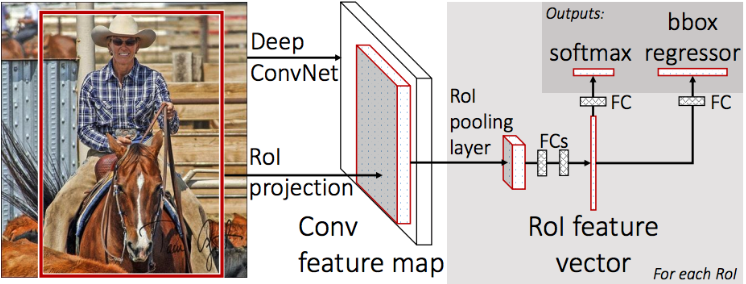
\includegraphics[width=0.9\textwidth]{SegundaEtapaR-CNN}
	\caption[Segunda etapa]{Segunda etapa \cite{segmentacionimagenes:marcoR-CNN}}
\end{figure}

\subsubsection{\textit{The Common Objects in Context} (COCO)}

Los datos de entrenamiento necesarios para realizar esta tarea requieren los objetos etiquetados con sus respectivas máscaras (o plantillas). De esta manera, es posible localizar automáticamente el objeto en la imagen. No existen muchas bases de datos públicas con este tipo de características.

Microsoft COCO \cite{segmentacionimagenes:COCO} es un conjunto de datos muy utilizado en segmentación de objetos. Contiene más de 200.000 imágenes etiquetadas y cerca de 80 clases diferentes.

Mask R-CNN \cite{segmentacionimagenes:MaskR-CNN2} ya proporciona pesos pre-entrenados para Microsoft COCO para empezar. Hemos utilizado estos pesos como punto de partida para entrenar la red por primera vez.

\section{\textit{Average Precision} (AP)\label{SectionAP}}

Antes de poder comprender AP (\textit{Average Precision}) o mAP (\textit{mean Average Precision}) \cite{AP}\cite{mAP}, primero debemos entender qué es precisión (\textit{precision}), sensibilidad o exhaustividad (\textit{recall}) y IoU (\textit{Intersection over union}).

\subsection{Precisión y sensibilidad}

\textbf{\textit{Precision}}: Mide cuán precisas son nuestras predicciones o la proporción de puntos de datos que nuestro modelo dice cuales son realmente relevantes. Es decir, que porcentaje de sus predicciones son correctas.

\textbf{\textit{Recall}}: Mide qué tan bueno es el modelo para encuentrar todos los puntos de datos de interés o casos relevantes.

Definiciones matemáticas:

\[Precision = \frac{TP}{TP + FP}\] \[Recall = \frac{TP}{TP + FN}\]

\begin{center}
    \textit{TP = True Positive      TN = True Negative}
    
    \textit{FP = False Positive      FN = False Negative}
\end{center}

Positivo (\textit{Positive}) o Negativo (\textit{Negative}): Se refiere a la predicción. Si el modelo predice 1 entonces será positivo, y se predice 0 será negativo.

Verdadero (\textit{True}) o Falso (\textit{False}): Se refiere si la predicción es correcta o no.

Hay que tener en cuenta que, si aumentamos la precisión, la sensibilidad disminuirá y viceversa.

\subsection{IoU (\textit{Intersection over union})}

IoU mide la superposición entre 2 límites. Lo usamos para medir cuánto se superpone nuestro límite predicho con la verdad del área (el límite del objeto real cuyas coordenadas se dan en el conjunto de entrenamiento). 

\begin{figure}[htb]
	\centering
	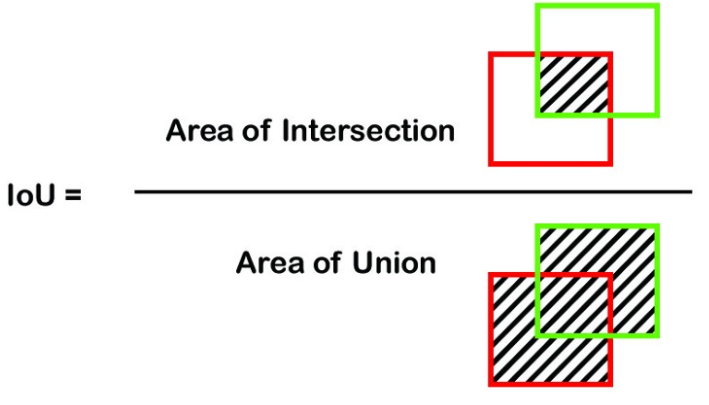
\includegraphics[width=0.7\textwidth]{IoU}
	\caption[Fórmula IoU]{Fórmula IoU \cite{AP}}
\end{figure}

Esto nos ayuda a clasificar si la predicción es un verdadero positivo (TP) o un falso positivo (FP). Con un valor umbral de 0.5 normalmente se clasifica de tres formas:

\begin{itemize}
    \item IoU > 0.5: Verdadero Positivo (TP).
    \item IoU < 0.5: Falso Positivo (FP).
    \item IoU > 0.5 Pero el objeto está clasificado erróneamente: Falso Negativo (FN).
\end{itemize}

En esta clasificación no hay un verdadero negativo (TN), esto es porque se supone que el cuadro delimitador siempre tendrá algo dentro, lo que significa que un cuadro delimitador nunca estará vacío.

\subsection{AP (\textit{Average Precision})}

Para empezar, necesitamos un conjunto de datos con las coordenadas reales de los defectos y las coordenadas predichas. Por ejemplo\footnote{Estos datos no son datos reales de las imágenes que tenemos. Son números aleatorios, pero con sentido.}:

\begin{table}[h]
	\begin{center}
		\begin{tabular}{l | c c}
			Imagen & Coordenadas reales & Coordenadas predichas\\ \hline
			Img1 & [123 233 183 367] & [130 253 169 370]\\
			Img2 & [276 202 454 310] & [341 209 466 295]\\
			Img3 & [378 204 456 266] & [372 211 460 268]\\
			Img4 & [309 101 429 343] & [325 157 409 361]\\
			Img5 & [71 252 163 348] & [26 275 160 371]\\
		\end{tabular}
		\caption{Conjunto de datos}
		\label{conjuntodedatos}
	\end{center}
\end{table}

A continuación, debemos calcular la precisión (\textit{precision}) y la sensibilidad (\textit{recall}). Tras calcular estos tres datos todavía quedaría un dato por calcular antes de calcular mAP, la precisión interpolada (\textit{Interpolated Precision} - IP).

\textbf{\textit{Interpolated Precision}}: se corresponde con el valor de precisión más alto para un determinado nivel de sensibilidad. Es decir, si tenemos el mismo valor de sensibilidad para tres valores de precisión diferentes 0.87, 0.76 y 0.68, entonces la precisión interpolada para los tres valores de sensibilidad será la más alta entre estos tres valores.

\[P_{interp}(r) = \max_{r'\geq r} p(r')\]

\newpage

Datos finales:

\begin{table}[h]
	\begin{center}
		\begin{tabular}{l | c c c c c}
			Imagen & IoU & TP/FP & Precision & Recall & IP\\ \hline
			Img1 & 0.550569 & TP & 1.000000 & 0.090909 & 1.000000\\
			Img2 & 0.482510 & FP & 0.500000 & 0.090909 & 1.000000\\
			Img3 & 0.774103 & TP & 0.666667 & 0.166667 & 0.666667\\
			Img4 & 0.513853 & TP & 0.750000 & 0.230769 & 0.750000\\
			Img5 & 0.430901 & FP & 0.600000 & 0.230769 & 0.750000\\
		\end{tabular}
		\caption{Datos finales}
		\label{datosfinales}
	\end{center}
\end{table}

Finalmente, dividimos el valor de sensibilidad de 0 a 1.0 en 11 puntos: 0, 0.1, 0.2, ... , 0.9 y 1.0. En nuestro ejemplo los valores máximo y mínimo son 0.230769 y 0.000000 respectivamente. Los valores serían: 0.000000, 0.0230769, 0.0461538, ... , 0.2076921, 0.230769. Con ello calculamos el promedio del valor de precisión máximo para estos 11 valores de sensibilidad.

\[AP = \frac{1}{11} \cdot (AP_{r}(0) + AP_{r}(0.1) + \ldots + AP_{r}(1.0))\]

En nuestro ejemplo,
\[AP = \frac{4 \cdot 1.000000 + 4 \cdot 0.666667 + 3 \cdot 0.750000}{11} = 0.810606\]